As the third use-case, we implemented the DVMS
proposal~\cite{quesnel:cpe2012}.
DVMS (Distributed Virtual Machine
Scheduler) is an algorithm that targets the dynamic scheduling of VMs hosted on
large-scale distributed infrastructure. It aims at preserving VMs QoS by
migrating VMs located on overloaded servers to underloaded ones. DVMS works in
a cooperative and fully distributed manner.

\subsubsection{Overview and Definitions}

Each node composing the infrastructure hosts a DVMS agent. Agents
are organized on top of an overlay network, which can be structured (such as
Chord ~\cite{stoica:2001:sigcomm01}) or unstructured.

When a server is overloaded (i.e. VMs hosted on the server consume resources
that can be produced), a scheduling procedure is started and a partition
containing nodes considered for the reconfiguration will grow. Initially, the
partition only contains the overloaded node.

Partitioning the infrastructure is mandatory to avoid conflicts between several
schedulers that could manipulate the same nodes or VMs when they apply their
reconfiguration plans.

Each partition includes two special nodes, the initiator and the leader.
The initiator of a partition is its initial node (i.e. the overloaded node).
The leader of a partition is the last node of the partition: it will lead the
scheduling computations, aiming at solving the overloading of the initiator;
In case of the scheduling computation is unsuccesful, a new node will be
inserted in the partition, becoming the new leader of the partition.


\subsubsection{Iterative Scheduling procedure}

When a node N\(_{\textit{i}}\) detects that it cannot provide enough resources
to its hosted VMs, it generates a partition and reserves itself to solve the
problem (see Figure~\ref{fig:dvms_pte_1}) : the node N\(_{\textit{i}}\) is the
initiator of the partition. After that, the partition is forwarded to its
closest neighbor N\(_{\textit{i+1}}\), given by the network overlay.

If N\(_{\textit{i+1}}\) is already involved in another partition, it directly
forwards the received partition to node N\(_{\textit{i+2}}\); otherwise,
N\(_{\textit{i+1}}\) joins the new partition (see Figure~\ref{fig:dvms_pte_2})
and checks that the scheduling procedure is still valid.  If the partition is
not valid anymore (for instance because VMs workload fluctuated),
N\(_{\textit{i+1}}\) cancels the reservations to destroy
the partition and thus allow the nodes that composed it to take part to an other
problem solving procedure.
%
On the contrary, if the procedure is still valid, N\(_{\textit{i+1}}\) notifies
members of the partition that it has become the new leader; in return, the new
leader receives information regarding (i)~the capacities of each node and
(ii)~the resources consumed by virtual machines that are hosted on each node.
The leader then starts a scheduling computation; if no solution is found, the
event is then forwarded to node N\(_{\textit{i+2}}\).

N\(_{\textit{i+2}}\) repeats the same procedure: self-reservation
(if it is free, see Figure~\ref{fig:dvms_pte_3}), event validity check, becoming
the leader, monitoring of VMs and nodes inside the partition and launching a
scheduling computation.  If N\(_{\textit{i+2}}\) finds a working reconfiguration
plan, it is applied in order to solve the overloading of the initator; Once the
application has been performed, the partition is dissolved and the nodes that
composed it are now able to take part to other problem solving procedures.

Note that, if N\(_{\textit{i+2}}\) did not find a solution, the partition would
have grown until a solution was found or the partition would have used all the
node constituting the infrastructure. In the latter case, the problem would be
considered as unsolvable and the partition would be destroyed.

The progressing increase in size of the partition aims at adapting it to the
complexity of the problem to solve.
This approach enables to consider as few nodes as possible, thus accelerating
the scheduling computations to solve the event as fast as possible.

% The problem solving procedure is initiated when a node
% N\(_{\textit{i}}\) observes that there is a problem, for instance when its
% resources are overused (see Figure~\ref{fig:dvms_pte}); it then generates an
% event and reserves itself to process this event (see
% Figure~\ref{fig:dvms_pte_1}).  After that, it forwards this event to its
% neighbor on the ring, node N\(_{\textit{i+1}}\).

% If N\(_{\textit{i+1}}\) is already involved in another partition, it directly
% forwards the event to node N\(_{\textit{i+2}}\); otherwise, N\(_{\textit{i+1}}\)
% joins the new partition (see Figure~\ref{fig:dvms_pte_2}) and checks that the
% event is still valid.  If the event is not valid anymore (for instance because
% the virtual machines demands for resources fluctuated), N\(_{\textit{i+1}}\)
% cancels the reservations to destroy the partition and thus allow the nodes that
% composed it to take part to other problem solving procedures.
% %
% On the contrary, if the event is still valid, N\(_{\textit{i+1}}\) notifies all
% the nodes inside the partition that it is the new leader; in return, it receives
% information regarding (i)~the capacities of each node and (ii)~the resources
% consumed by the virtual machines hosted on each node.  It then starts a
% scheduling computation; if no solution is found, the event is then forwarded to
% node N\(_{\textit{i+2}}\).

% N\(_{\textit{i+2}}\) repeats the same operations, that is to say: self-reservation
% (if it is free, see Figure~\ref{fig:dvms_pte_3}), event validity check, leader
% change notification, monitoring of VMs and nodes inside the partition,
% scheduling computation.  If N\(_{\textit{i+2}}\) finds a solution, it applies the
% corresponding reconfiguration plan that solves the event; it then cancels
% reservations to destroy the partition and thus allow the nodes that composed it
% to take part to other problem solving procedures.

% Note that, if N\(_{\textit{i+2}}\) did not find a solution, the partition would
% have grown until a solution was found or the even had traversed the whole ring.
% In the latter case, the problem would be considered as unsolvable and the
% partition would be destroyed.

% The progressing increase in size of the partition aims at adapting it to the
% complexity of the problem to solve.
% This approach enables to consider as few nodes as possible, thus accelerating
% the scheduling computations to solve the event as quickly as possible.

\begin{figure}[h]
\subfigure[]{
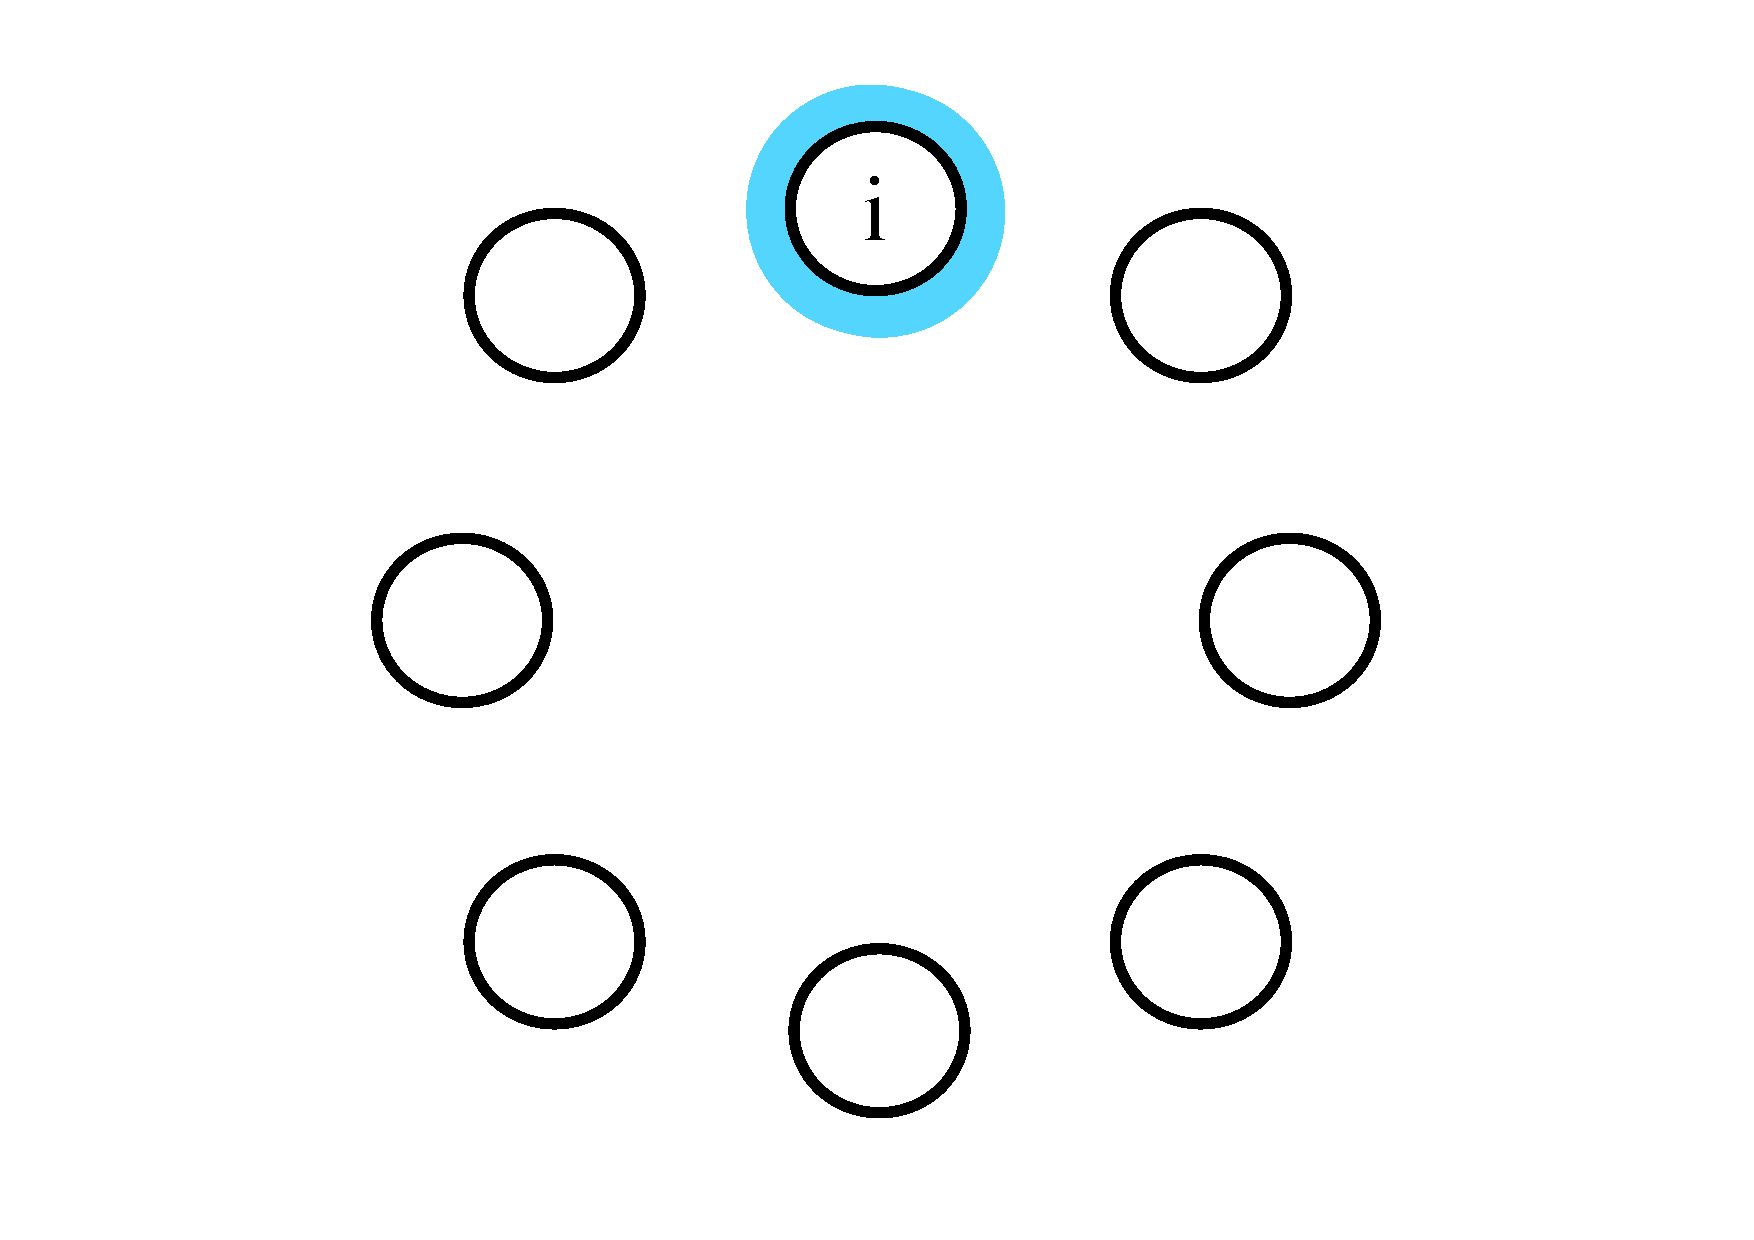
\includegraphics[width=3.8cm]{./figures/fig-24.pdf}
\label{fig:dvms_pte_1}}
%
\subfigure[]{
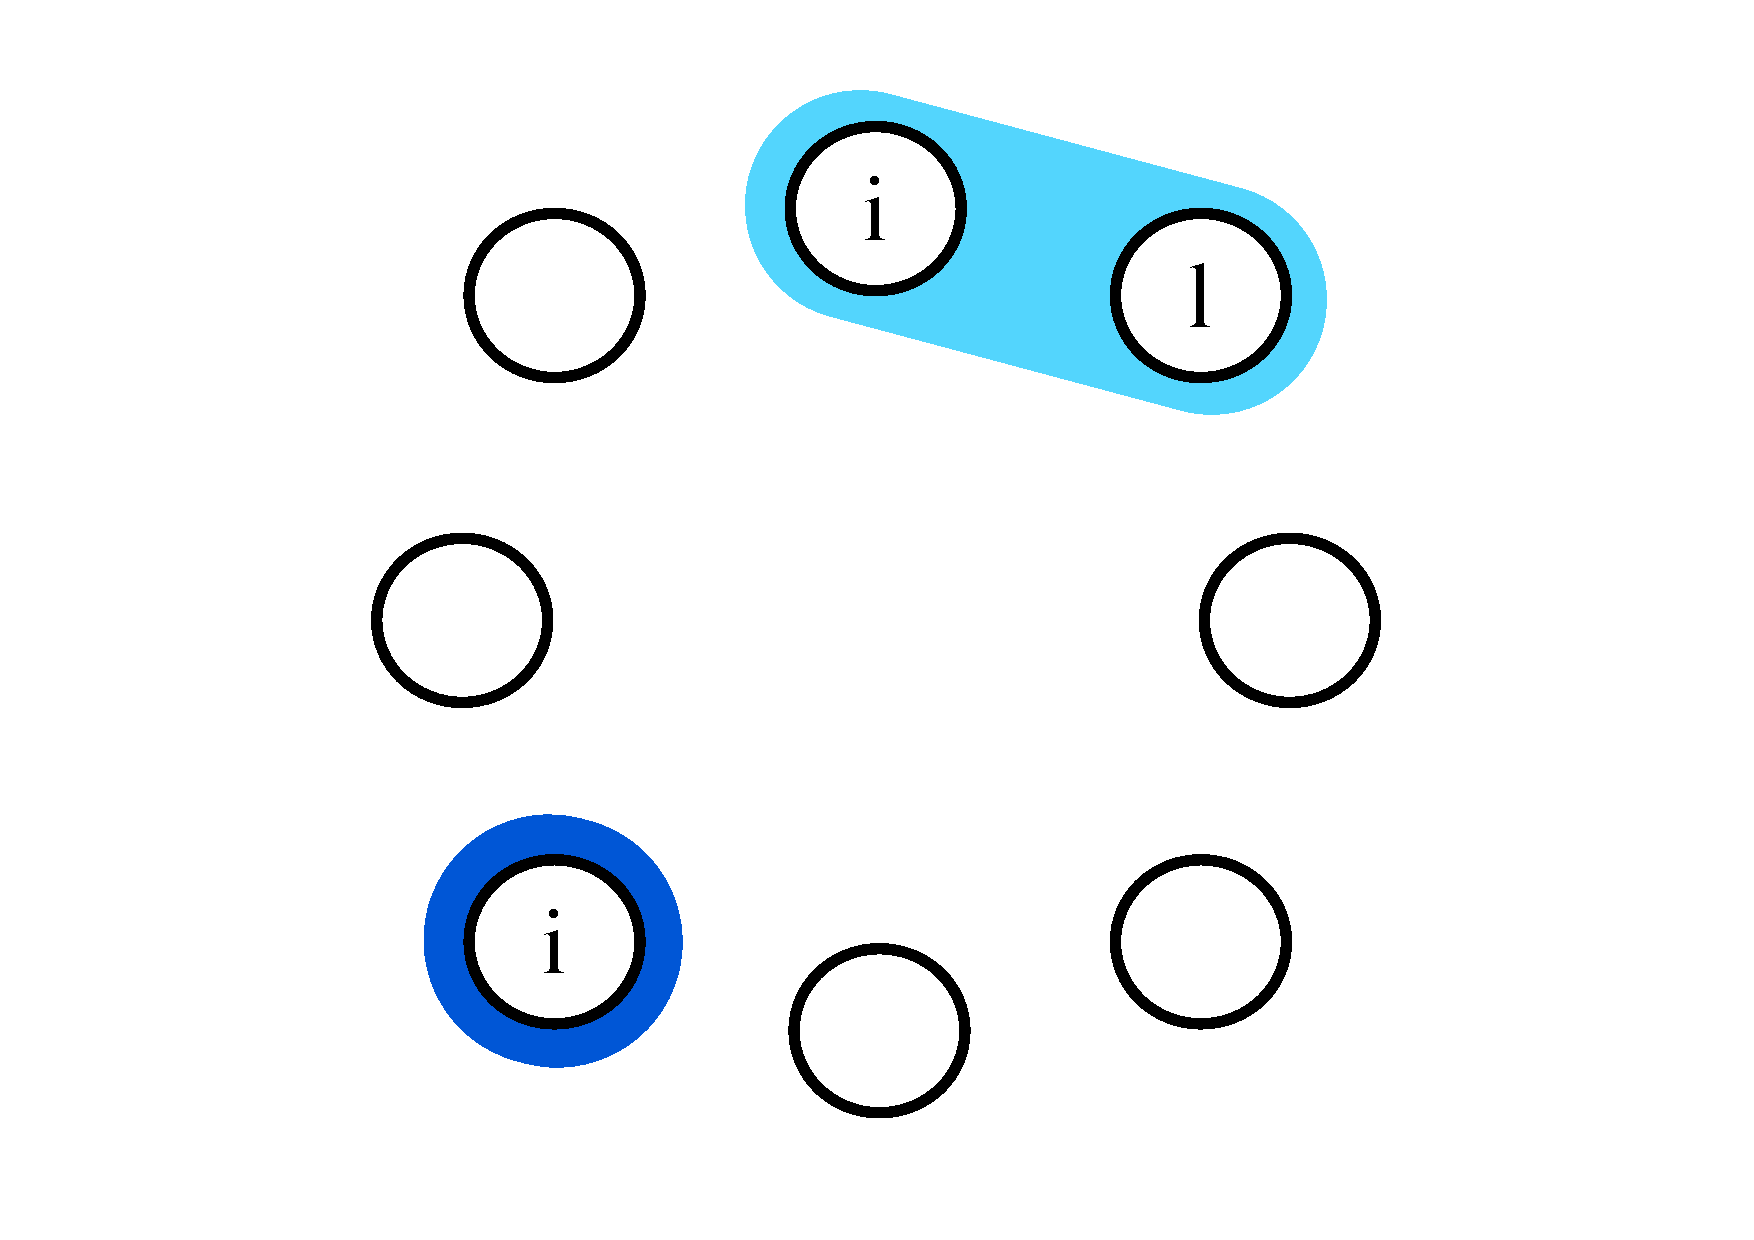
\includegraphics[width=3.8cm]{./figures/fig-25.pdf}
\label{fig:dvms_pte_2}}
%
\subfigure[]{
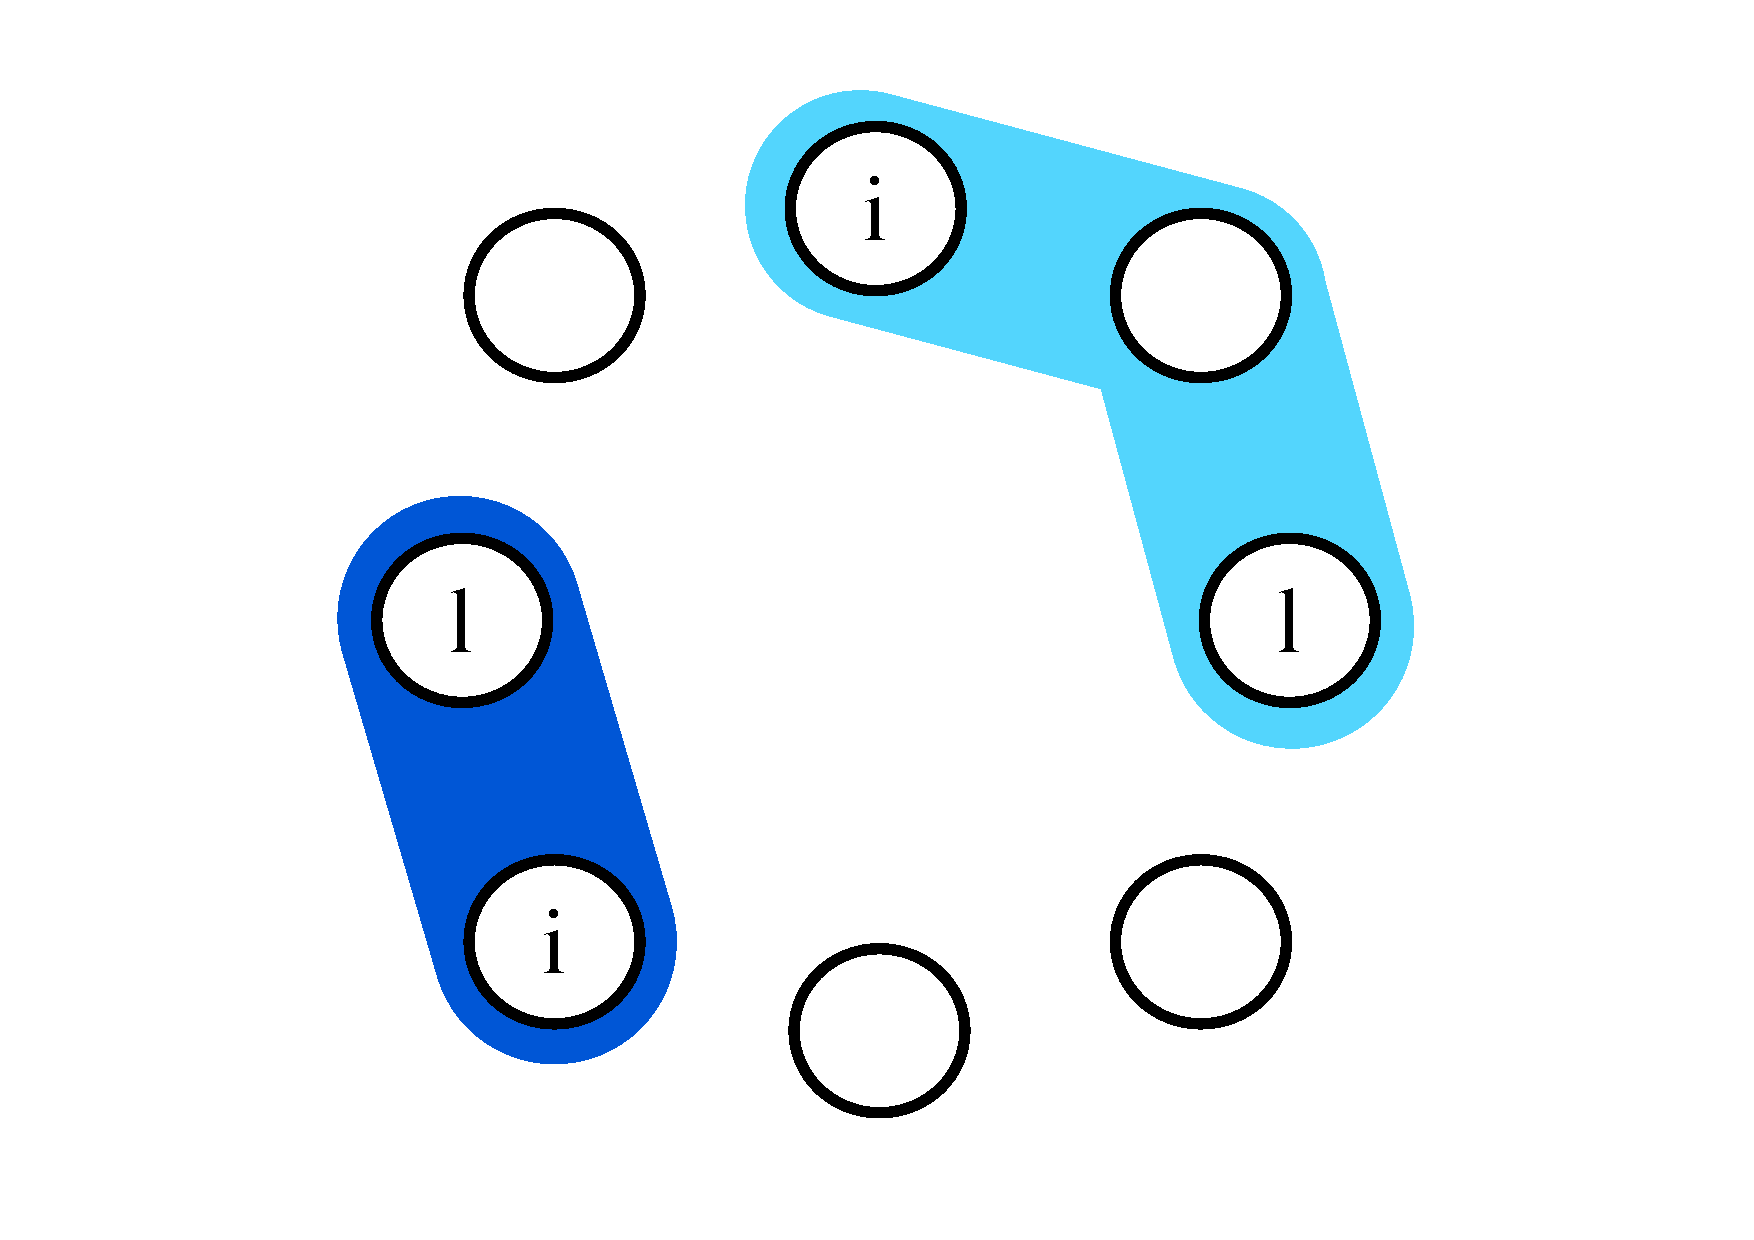
\includegraphics[width=3.8cm]{./figures/fig-26.pdf}
\label{fig:dvms_pte_3}}
%
\subfigure[Legend]{
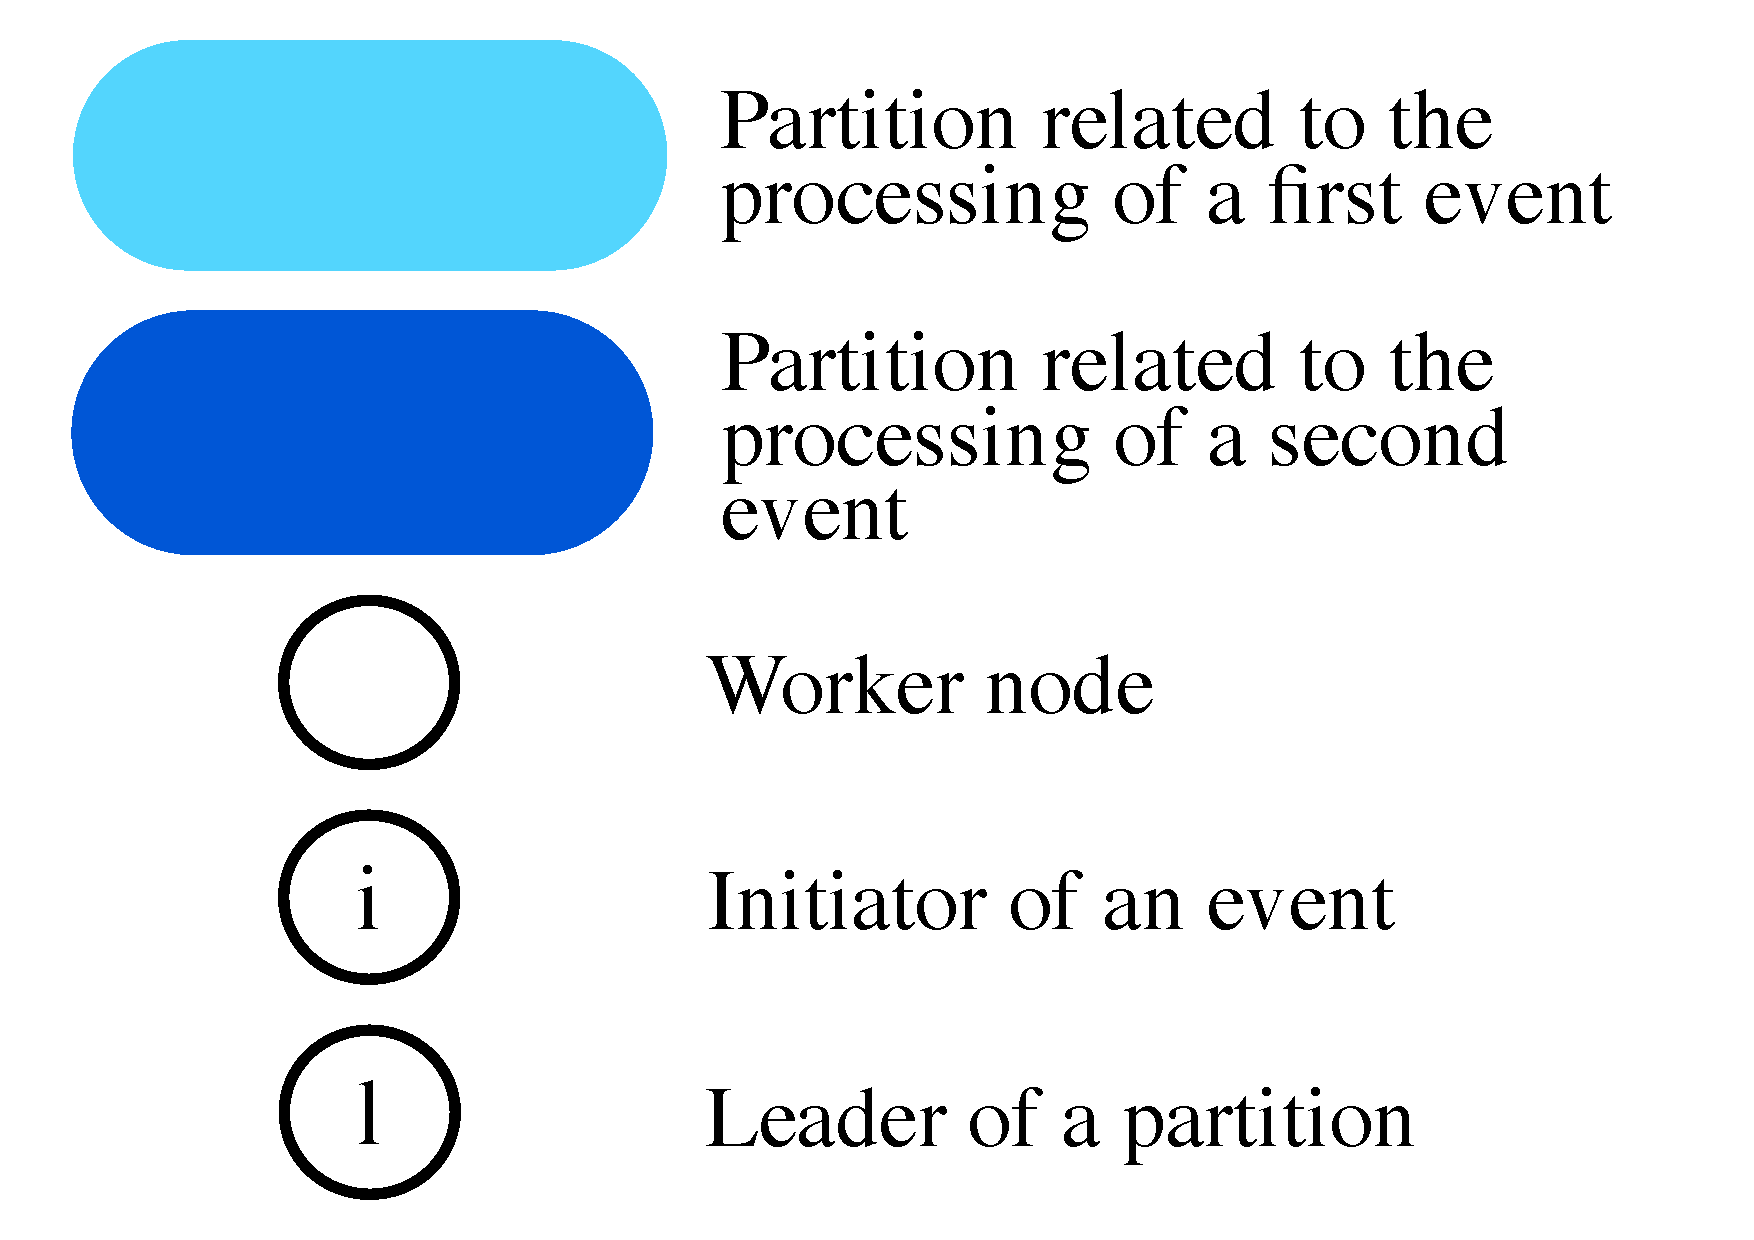
\includegraphics[width=3.8cm]{./figures/fig-27.pdf}
\label{fig:dvms_pte_4}}
%
\caption{Processing two events simultaneously\label{fig:dvms_pte}}
\end{figure}


\subsubsection{Fault-tolerance}

DVMS uses the inter-node collaboration: an overloaded node tries to find
underloaded nodes that may rebalance its load. As in large scale computing
nodes failures are frequent, DVMS includes fault tolerant mechanisms.



\paragraph{Using overlay networks.}

The main advantage of using overlay networks is that they have built-in fault
tolerance mechanisms. Thus, to manage the connectivity between its nodes, DVMS
works on top of an overlay network such as Chord: when a node needs to rebalance
its VMs workload, it asks the overlay network to find some collaborators. This
functionning allows firstly a loosely coupling between DVMS and the overlay
network used, and, secondly, to delegate most of the fault tolerance mechanisms
to the overlay network.


\paragraph{Destroying a Partition If One of Its Node Fails.}

Leveraging a fault-tolerant overlay network was not enough; it was also necessary to make the
problem solving procedure fault-tolerant.

Previously, if the leader of a partition crashed, the problem identified by the
initiator would never be solved; moreover, the nodes of this partition would
remain reserved indefinitely and would not be able to take part to other problem
solving procedures.

To avoid these issues, DVMS now relies on a timeout.  Each node involved in a
partition periodically checks whether the state of its partition changed
recently (for instance, a new node joined the partition).
%
If the state does not change anymore, it probably means that the problem solving
procedure is stuck (maybe because the leader crashed).
%
In this case, each node decides to leave the partition and becomes free to take
part to other problem solving procedures.
